\chapter{Conception de Gatling}
\label{chap_conception}

\section{Architecture de Gatling}
\subsection{Entrées \& sorties}
Gatling, comme tout programme informatique, accepte des données en entrée et renvoie des données en sortie. Les entrées sont créées par l'utilisateur de l'outil, tandis que les sorties sont destinées à être interprétées par ce même utilisateur. La figure \ref{io} représente les entrées et sorties de Gatling, elles sont composées de :

\begin{itemize}
  \item Entrées
  \begin{itemize}
	\item \em{Scripts}. Les scripts sont des fichiers scala qui contiennent les scénarios et simulations que le testeur veut exécuter.
  	\item \em{Seeds}. Les seeds\footnote{Graines en français} contiennent les données qui seront utilisées par les feeders\footnote{Voir section \ref{feeders} p.\pageref{feeders}} dans les scénarios.
  	\item \em{Bodies}. Les Bodies sont les corps envoyés avec les requêtes de type POST ou PUT.
  \end{itemize}
  \item Sorties
  \begin{itemize}
    \item \em{Rapports}. Les rapports générés au format HTML et également exportés en CSV
  \end{itemize}
\end{itemize}

\begin{figure}[h]
\begin{center}
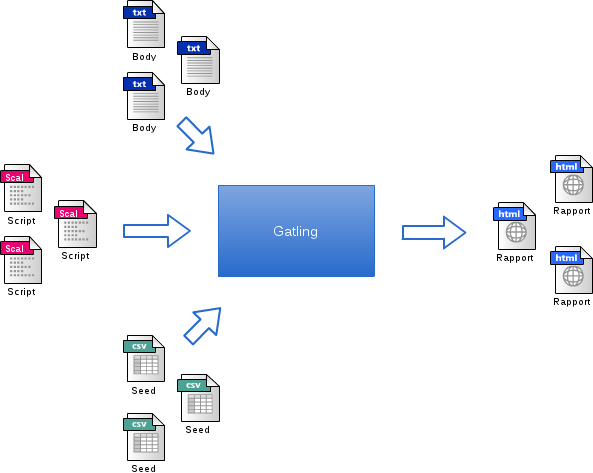
\includegraphics[width=400pt]{img/io.png}
\end{center}
\caption{Entrées et sorties de Gatling}
\label{io}
\end{figure}

\subsection{Application modulaire}
Gatling est découpé en différents modules interagissant les uns avec les autres. Ce découpage permet de créer des APIs\footnote{\en{Application Programmable Interface}. Les APIs sont des interfaces utilisables par d'autre logiciels afin d'utiliser celui qui les fournit} internes, ce qui facilite l'ajout de fonctionnalités similaires comme, par exemple, l'ajout du support d'un protocole autre que HTTP. La figure \ref{arch} montre les modules principaux nécessaires au test d'applications web standard et présents dans la première version de l'application :
\begin{itemize}
  \item \em{Gatling App}. C'est l'interface avec l'utilisateur de l'application, en l'occurence par la ligne de commande.
  \item \em{Gatling HTTP}. Ce module fournit les classes permettant de supporter le protocole HTTP.
  \item \em{Gatling Statistics}. Ce module fournit les classes permettant de générer les rapports.
  \item \em{Gatling Core}. Ce module contient toutes les fonctionnalités au coeur de l'application.
\end{itemize}

\begin{figure}[h]
\begin{center}
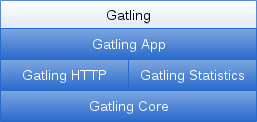
\includegraphics{img/arch.png}
\end{center}
\caption{Architecture de Gatling}
\label{arch}
\end{figure}

\subsection{Structure des dossiers}
Afin de permettre à l'application comme à l'utilisateur de savoir où se trouvent les fichiers nécessaires à l'exécution d'une simulation, une structure de dossiers a été créée. Cette structure est représentée ci-après par la figure \ref{folders}.

\begin{figure}[h]
\begin{center}
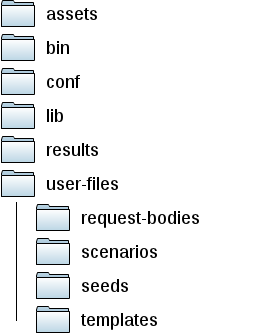
\includegraphics{img/folders.png}
\end{center}
\caption{Structure de dossiers de Gatling}
\label{folders}
\end{figure}

Le dossier \em{assets} contient des fichiers utiles à la génération des rapports. Les dossiers \em{bin} et \em{lib} contiennent les bibliothèques ainsi que l'exécutable qui permet de lancer Gatling. Le dossier \em{conf} contient le(s) fichier(s) de configuration de Gatling. Le dossier \em{results} contient les résultats de tests, rangés dans des dossiers portant comme nom la date et l'heure d'exécution du test.

Enfin, le dossier \em{user-files} contient les différents fichiers que l'utilisateur crée pour écrire ses scénarios. Le dossier \em{scenarios} contient les scripts écrits avec le DSL de Gatling. Le dossier \em{request-bodies} contient les corps de requête à être envoyés tels quels, alors que le dossier \em{template} contient des templates pouvant être complétés lors de l'exécution du scénario avant d'être envoyés. Le dossier \em{seeds} quant à lui contient les jeux de données utilisés par les feeders.

\section{Modules de l'application}
\subsection{Gatling App}
Ce module permet de proposer un menu au testeur, et ensuite, de charger dynamiquement les scripts correspondant à la simulation qui doit être exécutée. Une fois la simulation déroulée, la génération des rapports est exécutée et l'application s'arrête une fois que c'est terminé. Le menu proposé à l'utilisateur est montré sur la figure \ref{menu_console}.

\begin{figure}[h]
\begin{center}
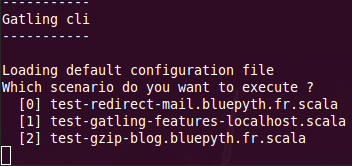
\includegraphics{img/menu_console.png}
\end{center}
\caption{Menu de sélection de la simulation à démarrer}
\label{menu_console}
\end{figure}

\subsection{Gatling Core}
\subsubsection{Présentation}
Ce module contient toutes les fonctionnalités au coeur de Gatling, et sert aussi de base aux autres en fournissant une API commune à tous les modules, notamment en ce qui concerne l'action \em{Request} qui servira de base pour tous les protocoles implémentés à l'avenir. Le schéma de la figure \ref{gatling_core} présente les divers composants de ce module.

\begin{figure}[h]
\begin{center}
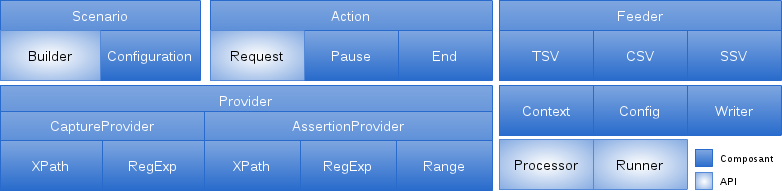
\includegraphics[width=400pt]{img/gatling_core.png}
\end{center}
\caption{Composants de Gatling Core}
\label{gatling_core}
\end{figure}

\subsubsection{Composants}
\label{sec_core_comp}
Les composants de Gatling Core sont les suivants :
\begin{description}
\item[Scenario] Il contient la définition d'un scénario et fournit l'API que doivent implémenter les modules qui souhaitent proposer une écriture de scénario qui leur est propre. Comme dans le reste de l'application, les composants \em{builder} servent à décrire le DSL, par souci de clarté, les autres ne sont pas représentés.
\item[Action] Au coeur du moteur, les actions sont en fait des acteurs au sens vu section \ref{sec_acteurs}.
\item[Feeder] Ce composant permet de lire les seeds que l'utilisateur a créées. Comme on le voit, il est possible de récupérer des informations depuis des fichiers CSV, TSV et SSV.
\item[Provider] Les providers sont les classes à la base des captures et des assertions. En effet, le fait d'avoir des providers dans Core permet de n'implémenter qu'une seule fois la recherche, mais de pouvoir l'utiliser dans tous les modules. Pour l'instant, il y a trois types de providers : RegExp (Expression Régulière), XPath et Range qui permet de vérifier qu'un nombre est bien compris entre deux valeurs\footnote{Ce provider permet de vérifier le statut des réponses entre 200 et 299 par exemple pour les réponses HTTP valides.}.
\item[Context] Ce composant permet de stocker ou récupérer des valeurs du contexte.
\item[Config] Composant permettant de lire la configuration utilisateur qui se trouve dans le fichier gatling.conf.
\item[Writer] Ce composant enregistre l'évolution des simulations dans un fichier.
\item[Processor] Cette API permet de définir des processors. Un processor est une unité qui agit sur la réponse. On y retrouve typiquement les captures et assertions, mais d'autres pourraient être ajoutés dans le futur.
\item[Runner] Cette API permet elle de définir la façon dont va s'exécuter le scénario.
\end{description}

\subsection{Gatling HTTP}
\subsubsection{Présentation}
Ce module permet d'utiliser Gatling pour tester des applications qui utilisent le protocole HTTP afin de communiquer, ce sont majoritairement des applications web. Les verbes HTTP supportés par ce module sont PUT, POST, GET et DELETE, ce qui rend possible le test d'applications RESTful et des webservices REST. Le schéma de la figure \ref{gatling_http} présente les divers composants de ce module.

\begin{figure}[h]
\begin{center}
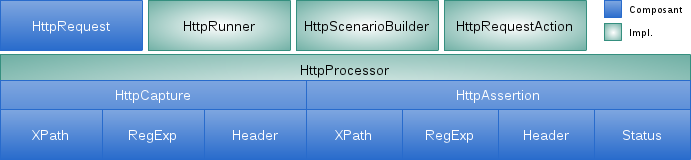
\includegraphics[width=400pt]{img/gatling_http.png}
\end{center}
\caption{Composants de Gatling HTTP}
\label{gatling_http}
\end{figure}

\subsubsection{Composants}
Les composants de Gatling HTTP sont les suivants :
\begin{description}
\item[HttpRequest] Ce composant est un wrapper de la classe Request du client HTTP utilisé : AsyncHttpClient\cite{www_ahc}. Elle permet, entre autres, de définir le DSL permettant de créer les requêtes HTTP.
\item[HttpRunner] Ce composant, comme expliqué dans la section \ref{sec_core_comp}, programme l'exécution des scénarios.
\item[HttpProcessor] Ce composant définit les captures et assertions qui pourront être utilisés sur les requêtes HTTP du scénario.
\end{description}

\subsection{Gatling Statistics}
\subsubsection{Présentation}
Ce module permet de générer les rapports de simulation et de calculer les statistiques nécessaires à ces mêmes rapports. Sa composition est présentée figure \ref{gatling_stats}. Il existe actuellement trois entités différentes pour lesquelles des statistiques sont calculées : les sessions, les requêtes d'un point de vue global et des détails pour chaque requête.

\begin{figure}[h]
\begin{center}
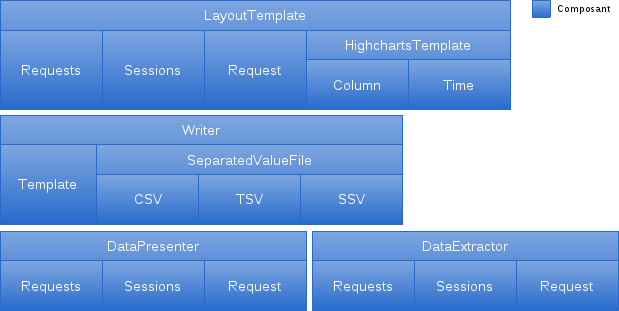
\includegraphics[width=400pt]{img/gatling_stats.png}
\end{center}
\caption{Composants de Gatling Statistics}
\label{gatling_stats}
\end{figure}

\vfill
\subsubsection{Fonctionnement}
Les statistiques sont générées selon le modèle de la figure \ref{stats_gen}. Lors de l'exécution du scénario, le moteur enregistre les résultats de chaque requête dans un fichier. Ce fichier est ensuite analysé par un \em{extracteur de données} qui récupère et formate les données utiles à la génération d'un graphique. Ces données sont ensuite mise en forme par les \em{presenters} et enfin, un fichier de rapport est créé au format HTML grâce à l'utilisation de templates, comme vu section \ref{sec_scalate}. En parallèle de la génération de rapports au format HTML, des fichiers au format TSV sont créés.

\begin{figure}[h]
\begin{center}
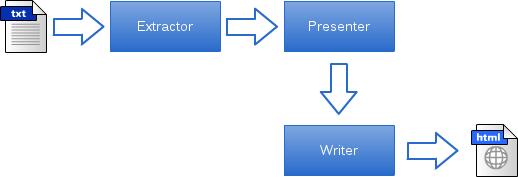
\includegraphics{img/stats_gen.png}
\end{center}
\caption{Génération de statistiques}
\label{stats_gen}
\end{figure}

La figure \ref{stats_exp} représente le résultat obtenu pour le détail d'une requête. On distingue deux graphiques : le premier indique le temps de réponse en fonction du temps, tandis que l'autre indique le nombre de requêtes par temps de réponse. Entre les deux graphiques, des données statistiques sont affichées telles que l'écart-type, la moyenne, la valeur maximale et minimale du temps de réponse, etc.

\begin{figure}[h]
\begin{center}
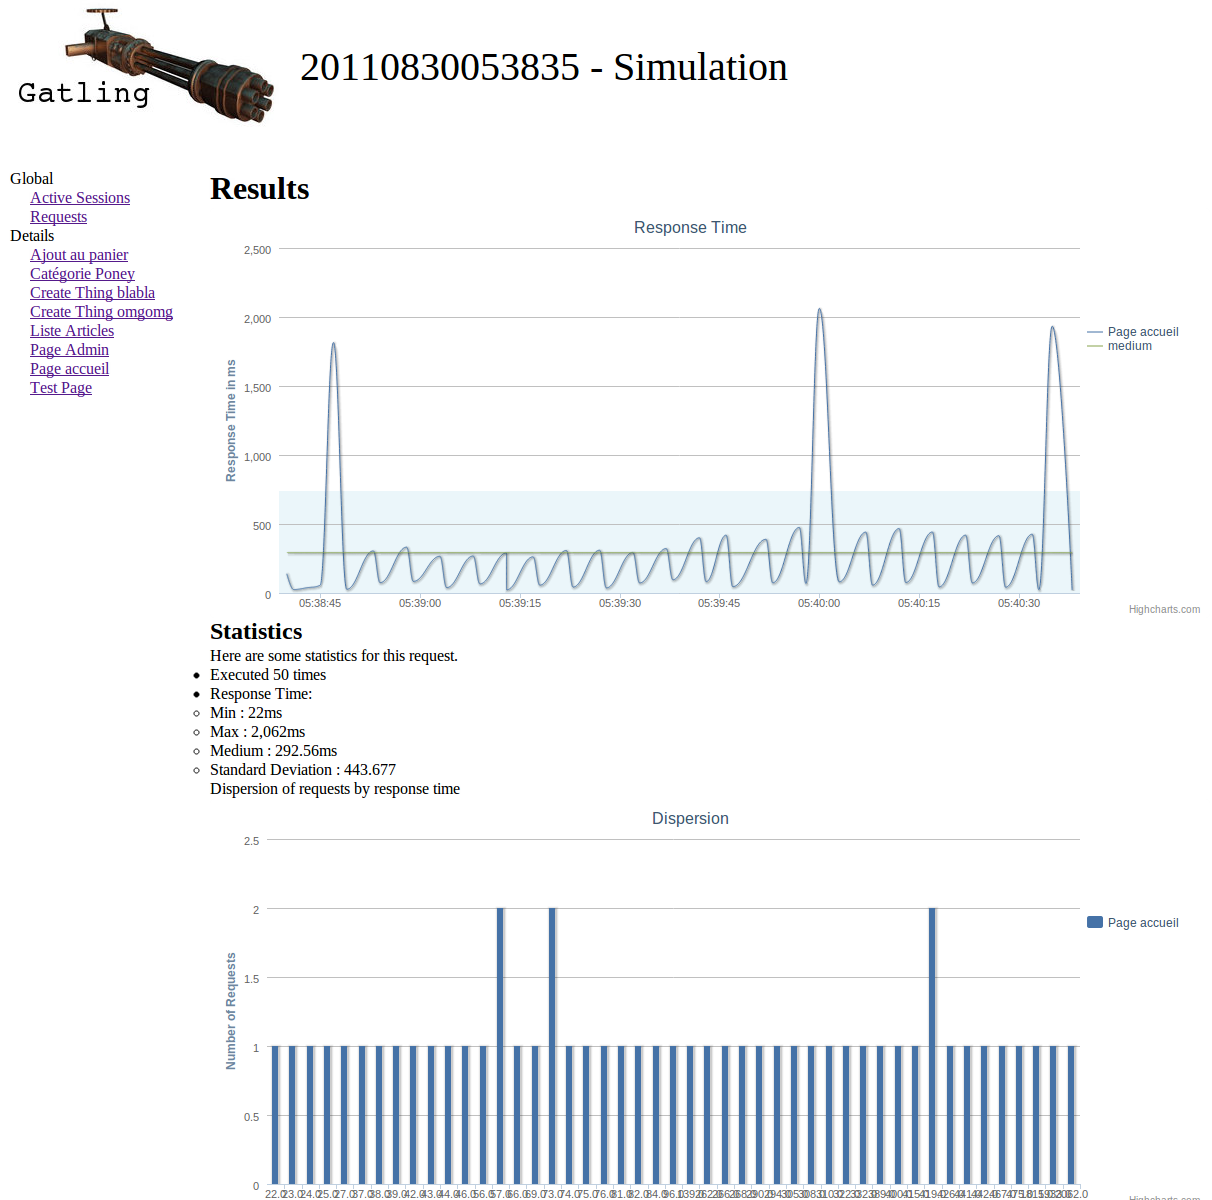
\includegraphics{img/stats_exp.png}
\end{center}
\caption{Exemple de statistiques générées}
\label{stats_exp}
\end{figure}

\section{Le DSL}
\subsection{Analyse d'un test de charge}
Afin de créer un DSL simple à utiliser, une analyse été faite afin de repérer les éléments que contiennent un scénario et une simulation.

\subsubsection{Définition d'un scénario}
Afin de définir un scénario d'utilisation, la personne qui l'écrit doit pouvoir spécifier :
\begin{itemize}
  \item Le nom du scénario ;
  \item Les requêtes faites par l'utilisateur, et pour chaque requête :
  \begin{itemize}
    \item Le type de la requête (HTTP pour l'instant) ;
	\item Le nom de la requête (pour facilement identifier la requête dans les statistiques) ;
    \item Le verbe HTTP utilisé (POST, PUT, GET ou DELETE) ;
    \item Les paramètres de la requête ;
    \item Le corps de la requête si possible ;
  \end{itemize}
  \item Les pauses qui simulent le temps de lecture de l'utilisateur.
\end{itemize}

\subsubsection{Exécution d'une simulation}
Une fois les scénarios écrits, il faudra les exécuter. Le testeur doit pouvoir configurer cette exécution. Voici les éléments configurables :
\begin{itemize}
  \item Le nombre d'utilisateurs simultanés pour ce scénario ;
  \item La rampe de démarrage des utilisateurs. Ceci permet de simuler un arrivage progressif des utilisateurs sur le site par exemple ;
  \item Le démarrage du scénario. En effet, plusieurs scénarios peuvent être exécutés durant une simulation, on peut donc spécifier à quel moment de la simulation le scénario doit débuter.
\end{itemize}

\subsection{Définition du DSL}
Les éléments que l'analyse a permis de découvrir représentent la base du DSL. Pour chaque élément, vous trouverez un exemple du DSL qui correspond. Le logiciel étant Open Source et destiné aux entreprises du monde entier, le DSL est en anglais.

\subsubsection{Déclaration d'une requête HTTP}

Le DSL permet de déclarer et configurer facilement des requêtes HTTP. Le code du listing \ref{declare_request} montre quelques unes des diverses possibilités offertes. 

\begin{lstlisting}[caption={Déclaration d'une requête HTTP},label={declare_request}]
// Faire une requete de type GET sur l'url http://google.fr
get("http://google.fr")

// Faire une requete de type GET sur 
// l'url http://google.fr?q=ma+recherche
get("http://google.fr") withQueryParam ("q", "ma+recherche")

// Faire une requete de type POST sur l'url http://monurl.com
// avec le corps : '{"mon_object": {"attribut": "valeur" }'
// et des headers specifiant le contenu : JSON
post("http://monurl.com")
   withBody """{ "mon_object" : { "attribut": "valeur" }"""
   asJSON

// Faire une requete de type PUT sur l'url http://monurl.com
// avec le parametre de formulaire 'name' = 'John'
put("http://monurl.com") withParam ("name", "John")
\end{lstlisting}

\subsubsection{Déclaration d'un scénario}

L'exemple suivant, montré dans le listing \ref{declare_scenario}, illustre la façon dont un scénario peut être créé via le DSL de Gatling. Un scénario basique permettant de tester une application web contient des requêtes de type HTTP, ainsi que des pauses permettant de simuler le temps de lecture de l'utilisateur.

\begin{lstlisting}[caption={Déclaration d'un scénario simple},label={declare_scenario}]
// Declarer un scenario nomme 'S1', constitue d'une requete 
// sur le site de Google, attendre 1 seconde puis executer 
// une requete de recherche.
scenario("S1")
  doHttpRequest("Accueil", get("http://google.fr"))
  pause(1)
  doHttpRequest("Recherche", get("http://google.fr") 
    withQueryParam ("q", "keyword")
\end{lstlisting}

\subsubsection{Déclaration d'une simulation}

La dernière étape, une fois le scénario écrit, consiste à le configurer pour l'exécuter. Le listing \ref{declare_all} montre de quelle façon est déclarée la configuration puis la demande d'exécution de la simulation.

\begin{lstlisting}[caption={Déclaration d'une simulation au complet},label={declare_all}]
// On declare un scenario
val stdUser = scenario("Standard") do...

// On cree une configuration pour ce scenario avec
// * 5 utilisateurs concurrents
// * 0 seconde de rampe
// * 0 seconde de delai au demarrage
val stdUserConf = 
  configureScenario(stdUser)
    withUsersNumber 5 
    withRamp 0
    startsAt 0
val execution = runSimulations(stdUserConf)
\end{lstlisting}

\subsection{Fonctionnalités supplémentaires du DSL}
Afin de simplifier l'écriture des scénarios et d'augmenter les possibilités du DSL, des fonctionnalités supplémentaires ont été ajoutées.

\subsubsection{Captures et assertions}
Afin de valider les requêtes, le testeur pourra utiliser des assertions sur la réponse HTTP, permettant de vérifier son code, ainsi que la présence de certains \em{headers} ou des expressions dans le corps de la réponse. Cela permettra par exemple de valider une requête de login avant d'exécuter le reste du scénario. 

Les assertions sont basées sur les captures qui permettent de faire des recherches par expression régulière ou par XPath. Ces captures sont exécutées sur la réponse HTTP reçue par le moteur de simulation. Chacun de ces \em{processeors} est disponible indépendamment de l'autre dans le DSL, le listing \ref{use_capture_and_assertion} montre comment ils sont utilisés.

\begin{lstlisting}[caption={Utilisation des captures et assertions},label={use_capture_and_assertion}]
scenario("S1")
  doHttpRequest(
    "Accueil",
    get("http://www.google.fr"),
    // On stocke "ou" dans "name"
    regexp("""Ab(.*)t""") in "name",
    // On verifie qu'on est bien sur google
    assertRegexp("""<img alt="(.*)" """, "Google")
  )
\end{lstlisting}

\subsubsection{Contexte}
Un contexte est propre à un seul utilisateur simulé par un scénario. La présence de ce contexte permet au testeur de faire passer des infos de requêtes en requêtes.

Le testeur pourra extraire des données des réponses HTTP afin de les stocker dans le contexte, cela se fera en utilisant des captures (ou des assertions), les valeurs seront ensuite accessibles dans le reste du scénario. Le listing \ref{use_context} montre l'utilisation du contexte dans le cadre d'un scenario simple.

\begin{lstlisting}[caption={Utilisation du contexte},label={use_context}]
scenario("S1")
  doHttpRequest(
    "Set Value",
    get("http://google.fr"),
    regexp("""<img alt="(.*)" """) in "pagename")
  pause(1)
  doHttpRequest(
  	"Use value",
  	get("http://google.fr") 
  	  withQueryParam ("q", FromContext("pagename")))
\end{lstlisting}

\subsubsection{Feeders (ou Seeders)}
\label{feeders}
La simulation d'un grand nombre d'utilisateurs peut nécessiter l'utilisation d'un nombre aussi grand de comptes différents sur l'application testée. Pour permettre l'utilisation d'un compte différent par utilisateur simulé, Gatling propose des Feeders\footnote{ou Seeders, le nom n'étant pas encore figé}. Ces éléments permettent d'utiliser une source de données telles qu'un fichier de type CSV pour y récupérer des informations à utiliser dans le scénario. Le listing \ref{use_feeder} montre l'utilisation de ces Feeders dans le cadre d'un scénario simple.

\begin{lstlisting}[caption={Utilisation des Feeders},label={use_feeder}]
// Declaration du Feeder
userCredentials = 
  new CSVFeeder("user_cred", List("login", "password"))

scenario("S1")
  doHttpRequest(
    "Login",
    post("http://mywebsite.com/login")
      // Declaration du Feeder pour cette requete
      withFeeder userCredentials
      // Utilisation des parametres du feeder
      withParam "login"
      withParam "password"
\end{lstlisting}